\documentclass[format=acmsmall, review=false, screen=true]{acmart}

\renewcommand{\texttt}[1]{%
  \begingroup
  \ttfamily
  \begingroup\lccode`~=`/\lowercase{\endgroup\def~}{/\discretionary{}{}{}}%
  \begingroup\lccode`~=`[\lowercase{\endgroup\def~}{[\discretionary{}{}{}}%
  \begingroup\lccode`~=`.\lowercase{\endgroup\def~}{.\discretionary{}{}{}}%
  \catcode`/=\active\catcode`[=\active\catcode`.=\active
  \scantokens{#1\noexpand}%
  \endgroup
}

\usepackage{booktabs} % For formal tables
\usepackage{tikz}
\usetikzlibrary{positioning,fit,calc,shapes,shadows,arrows}
\usepackage{forest}
\usetikzlibrary{arrows.meta}
\usepackage[ruled]{algorithm2e} % For algorithms
\renewcommand{\algorithmcfname}{ALGORITHM}
\SetAlFnt{\small}
\SetAlCapFnt{\small}
\SetAlCapNameFnt{\small}
\SetAlCapHSkip{0pt}
\IncMargin{-\parindent}
\usepackage{hyperref}
\usepackage[normalem]{ulem}

% Metadata Information
\acmJournal{TOSEM}
%\acmVolume{}
%\acmNumber{}
%\acmArticle{}
%\acmYear{}
%\acmMonth{}
\copyrightyear{2018}
%\acmArticleSeq{9}

% Copyright
%\setcopyright{acmcopyright}
\setcopyright{acmlicensed}
%\setcopyright{rightsretained}
%\setcopyright{usgov}
%\setcopyright{usgovmixed}
%\setcopyright{cagov}
%\setcopyright{cagovmixed}

% DOI
\acmDOI{0000001.0000001}

% Paper history
%\received{February 2007}
%\received[revised]{March 2009}
%\received[accepted]{June 2009}

\newcommand{\dl}{drasil-lang}
\newcommand{\dc}{drasil-code}
\newcommand{\dd}{drasil-data}
\newcommand{\de}{drasil-example}
\newcommand{\dg}{drasil-gen}
\newcommand{\drp}{drasil-printers}
\newcommand{\ddl}{drasil-docLang}

\newcommand{\edl}{\emph{\dl}}
\newcommand{\edc}{\emph{\dc}}
\newcommand{\edd}{\emph{\dd}}
\newcommand{\ede}{\emph{\de}}
\newcommand{\edg}{\emph{\dg}}
\newcommand{\edp}{\emph{\drp}}
\newcommand{\eddl}{\emph{\ddl}}

%% Comments
\newif\ifcomments\commentstrue

\ifcomments
\newcommand{\authornotes}[3]{\textcolor{#1}{[#3 ---#2]}}
\newcommand{\todo}[1]{\textcolor{red}{[TODO: #1]}}
\else
\newcommand{\authornotes}[3]{}
\newcommand{\todo}[1]{}
\fi

\newcommand{\wss}[1]{\authornotes{blue}{SS}{#1}}
\newcommand{\jc}[1]{\authornotes{red}{JC}{#1}}
\newcommand{\ds}[1]{\authornotes{olive}{DS}{#1}}

% Document starts
\begin{document}

%%%%%%%%%%%%%%%%%%%%%
% Tikz Styles
\tikzstyle{class}=[rectangle, draw=black, rounded corners, fill=white!40, drop 
shadow,
text centered, anchor=north, text=black, text width=3cm]
\tikzstyle{myarrow}=[->, >=triangle 90, thick]
%%%%%%%%%%%%%%%%%%%%%

% Title portion. Note the short title for running heads
\title[headertitle]{TITLE}

\author{Dan Szymczak}
%\orcid{1234-5678-9012-3456}
\affiliation{%
  \institution{McMaster University}
  \streetaddress{1280 Main St. W.}
  \city{Hamilton}
  \state{ON}
  \postcode{L8S 4K1}
  \country{Canada}}
\email{szymczdm@mcmaster.ca}
\author{Jacques Carette}
%\affiliation{%
%  \institution{Inria Paris-Rocquencourt}
%  \city{Rocquencourt}
%  \country{France}
%}
%\email{beranger@inria.fr}
\author{Spencer Smith}
%\affiliation{%
% \institution{Rajiv Gandhi University}
% \streetaddress{Rono-Hills}
% \city{Doimukh}
% \state{Arunachal Pradesh}
% \country{India}}
%\email{aprna_patel@rguhs.ac.in}
%\author{Huifen Chan}
%\affiliation{%
%  \institution{Tsinghua University}
%  \streetaddress{30 Shuangqing Rd}
%  \city{Haidian Qu}
%  \state{Beijing Shi}
%  \country{China}
%}
%\email{chan0345@tsinghua.edu.cn}
%\author{Ting Yan}
%\affiliation{%
%  \institution{Eaton Innovation Center}
%  \city{Prague}
%  \country{Czech Republic}}
%\email{yanting02@gmail.com}
%\author{Tian He}
%\affiliation{%
%  \institution{University of Virginia}
%  \department{School of Engineering}
%  \city{Charlottesville}
%  \state{VA}
%  \postcode{22903}
%  \country{USA}
%}
%\affiliation{%
%  \institution{University of Minnesota}
%  \country{USA}}
%\email{tinghe@uva.edu}
%\author{Chengdu Huang}
%\author{John A. Stankovic}
%\author{Tarek F. Abdelzaher}
%\affiliation{%
%  \institution{University of Virginia}
%  \department{School of Engineering}
%  \city{Charlottesville}
%  \state{VA}
%  \postcode{22903}
%  \country{USA}
%}


\begin{abstract}

CONTEXT: Software (re-)certification requires the creation and maintenance of
many different software artifacts. Manually creating and maintaining \wss{and
reusing?} them is tedious and costly. \wss{and error prone}

OBJECTIVE: Improve software (re-)certification efforts by automating as much of
the artifact creation process as possible, while maintaining full traceability
within -- and between -- artifacts.  %DS Secondary objective -> Knowledge reuse 
%-- Don't know if I want
% to focus here as it muddies the waters.

METHOD: %Use grounded theory in the creation of a tool for software artifact
%generation. 
Start by analyzing the artifacts themselves from several case 
studies to understand what (semantically) is being said in each.
Capture the underlying knowledge and apply transformations to create each of 
the requisite artifacts through a generative approach.  

RESULTS: Case studies -- GlassBR to show capture and transformation. SWHS and
NoPCM for reuse (Something about Kolmogorov complexity / MDL here?).
% Moved from Method:
Captured knowledge can 
be re-used across projects as it represents the ``science''. Maintenance
involves updating the captured knowledge or transformations as necessary.
%Moved from Objective:
Creation of our tool -- Drasil -- facilitates this automation process using a 
knowledge-based approach to Software Engineering.  \wss{Maybe add something
  about the infrastructure now being in place to reuse/grow the scientific and
  computing knowledge base to cover new case studies?  It would be nice if we
  could make the connection between Drasil's knowledge and existing scientific
  knowledge ontologies \ds{like which?}, but maybe it is too early for that 
  connection?}

CONCLUSIONS: With good tool support and a front-loaded time investment, we can 
automate the generation of software artifacts required for certification. 
(fill in later)?????

\wss{The abstract doesn't have anything from Jacques ``bottom up'' viewpoint.
  Can you work in something about consistency by construction?}

\end{abstract}


%
% The code below should be generated by the tool at
% http://dl.acm.org/ccs.cfm
% Please copy and paste the code instead of the example below.
%
%\begin{CCSXML}
%<ccs2012>
% <concept>
%  <concept_id>10010520.10010553.10010562</concept_id>
%  <concept_desc>Computer systems organization~Embedded systems</concept_desc>
%  <concept_significance>500</concept_significance>
% </concept>
% <concept>
%  <concept_id>10010520.10010575.10010755</concept_id>
%  <concept_desc>Computer systems organization~Redundancy</concept_desc>
%  <concept_significance>300</concept_significance>
% </concept>
% <concept>
%  <concept_id>10010520.10010553.10010554</concept_id>
%  <concept_desc>Computer systems organization~Robotics</concept_desc>
%  <concept_significance>100</concept_significance>
% </concept>
% <concept>
%  <concept_id>10003033.10003083.10003095</concept_id>
%  <concept_desc>Networks~Network reliability</concept_desc>
%  <concept_significance>100</concept_significance>
% </concept>
%</ccs2012>
%\end{CCSXML}

%\ccsdesc[500]{Computer systems organization~Embedded systems}
%\ccsdesc[300]{Computer systems organization~Redundancy}
%\ccsdesc{Computer systems organization~Robotics}
%\ccsdesc[100]{Networks~Network reliability}

%
% End generated code
%


\keywords{??}


\maketitle

% The default list of authors is too long for headers.
\renewcommand{\shortauthors}{D.\ Szymczak et al.}
\newcommand{\fgr}{\textcolor{red}{!FIGURE!}}
\section{Introduction}\label{S:Intro}

Writing non-executable software artifacts (requirements and design documents,
verification \& validation plans, etc.) can be tedious work, but is 
ultimately necessary when attempting to certify software. 
Similarly, maintenance of these artifacts, as necessary for re-certification as 
improvements are made, typically requires a large time investment.

Why, in a world of software tools, do we continue to undertake these
efforts manually? Literate programming had the right idea, but was too heavily 
focused on code.

We want to aid software (re-)certification efforts by automating as much of the 
artifact creation process as possible. By generating our software artifacts -- 
including code -- in the right way, we can implement changes much more quickly 
and easily for a modest up-front time investment. By front-loading the costs of 
maintenance and rolling them into the development cycle, we can save time and 
money in the long run.

\wss{The above is true, but only after the investment in building the generator
  infrastructure and incorporating the required knowledge.  Based on a
  discussion with JC, and some of his original text, I recently wrote a little
  blurb about this effort.  You could probably modify this to work in your paper
  somewhere.  ``The proposed work can improve the quality of SCS and reduce the cost of its
development, but this will require a transformative change in development
practices.  Using Drasil for an SCS project will require a willingness to encode
all of the knowledge, both declarative and procedural, about the relevant topics
inside Drasil.  Although encoding this information is a significant undertaking,
the payoff is potentially enormous -- We get to generate fully-documented
families of programs at an incrementally tiny cost.  The large up-front
investment has a large long-term payoff.  Current software development, has a
small up-front cost, and ever-increasing maintenance costs to continue.  Drasil
will completely change this effort curve.''}

\wss{The bottom up justification should also be part of the introduction.}

\ds{bottom up justification can go here?} \wss{You mention a table below
  (Problems and Proposed Solutions).  That would be the spot to discuss the
  bottom up justification.  To make sure we are communicating about the same
  thing, when I say bottom up justification, I'm talking about consistency.}

We \ds{and others -- citation ?} have observed a number of issues arise 
throughout a standard software development and maintenance life-cycle.
Information duplication is a major concern as several problems occur therein. 
The first, most trivial, and incredibly tedious is that of the necessity to 
duplicate information across software artifacts. A piece of knowledge that 
appears in the Software Requirements Specification (SRS) will undoubtedly 
appear in the design and implementation artifacts (documents/source code). This 
knowledge \emph{may} be transformed, but in many cases is an exact copy 
(Ctrl-C \& Ctrl-V anyone?) and a 
massive waste of time for a human to replicate throughout multiple 
artifacts.

Duplication also becomes a time-sink for maintenance, particularly as the 
duplicated information tends to fall out of sync across artifacts over the 
course of a piece of software's lifetime. For example, a common problem is that 
of updating the source code, but not updating any of the design documents to 
reflect the change. These inconsistencies are at best a minor headache and at 
worst, in the case of software certification, an expensive lesson. If the 
artifacts are inconsistent when submitted for (re-)certification, the software 
will not be (re-)certified and an extra cost will be incurred (both in labour, 
and from the certifying body) to attempt certification again.

\ds{Fill in this part about consistency, variabilities, and commonalities}

\begin{table}
	\caption{Problems and Proposed Solutions}
	\label{Tab:ProbSol}
	\begin{tabular}[width=0.5\textwidth]{l | l}		
		Problem 		& Technical Solution 					\\
		\hline
		Duplication		& Databases (global \& system-specific) \\
						& single-source \& generation *			\\
		\hline
		Consistency 	& 	Sanity checkers						\\
		(incl. Source/	& 										\\
		generated content)	&  									\\
		\hline
		Variability \&	& Software families \& 					\\
		Commonality		& Generation							\\
	\end{tabular}

\textit{* Also provides free \& easy reuse}
\end{table}

Table~\ref{Tab:ProbSol} gives a brief rundown of our proposed solutions to the 
problems mentioned above. We are leveraging our experience with generative 
programming to provide a solution that is applicable to a wide range of 
problems. \wss{This blurb about the table isn't enough to explain its content.}

%DS Maybe throw in a figure here to show off a bunch of common artifacts.

%DS Should everything after this point go into Background? Maybe not

\wss{We can certainly wait to do it, but I like a ``roadmap'' paragraph at the
  end of the introduction.  The roadmap explains how the paper is organized.
  More importantly, it provides an opportunity to present your ``story,''
  assuming that the organization of the paper follows the story.}

\subsection{Software (Re-)certification}

When we talk about software certification, we are specifically discussing the 
goal of determining ``based on the principles of science, engineering and 
measurement theory, whether an artifact satisfies accepted, well defined and 
measurable criteria''~\cite{HatcliffEtAl2009}. Essentially, we are ensuring 
that software, or some piece of it, performs a given task to within an 
acceptable standard and can potentially be reused in other systems.

Software certification is necessary by law in certain fields. This is 
particularly evident in safety-critical applications such as control systems 
for nuclear power plants or X-ray machines. 

Different certifying bodies exist across domains and each has their own list of 
requirements to satisfy for certifying software. Looking at some 
examples \cite{CSA1999,CSA2009,CDRH2002,FDA2014} there are many pieces
of requisite documentation including, but not limited to:

\begin{itemize}
\item Problem definition
\item Theory manual
\item Requirements specification
\item Design description
\item Verification and Validation (V\&V) report
\end{itemize}

We should keep in mind that we require full traceability -- inter- and 
intra-artifact -- of the knowledge contained within these artifacts. That is, 
we should be able to find an explicit link between our problem definition and 
theory manual, down to our requirements, design, and other development planning 
artifacts. From there, we should be able to continue through our proposed 
verification and validation plans, and should eventually end up in the V\&V 
report. \wss{Why do we require full traceability.  I agree, but you should tell
  the reader why this documentation quality is so important.}

\ds{rework the following paragraph} \wss{I agree - you say it is expensive two
  different ways.  You only need to say it once.  :-)}
Ensuring this traceability and, in fact, getting anything certified has many 
costs associated with it. There is a massive time investment, fees, and costs 
associated with contracting out a third-party verifier. Overall it is a 
very expensive process.

Re-certification of software following any change, no matter how minor, %DS 
%keep?
incurs a similar level of costs; all the artifacts must be updated to 
reflect the new change, and everything must be re-checked and verified to 
ensure no new errors have been introduced. We have an implicit burden of 
ensuring the consistency of related information across our artifacts.

We intend to alleviate some of this cost-burden through a strategic, generative 
approach to Software Engineering (SE). With the automated generation of 
artifacts we can ensure they are \emph{consistent by construction}, implement 
changes 
quickly, and automatically update relevant and/or dependent artifacts.  \wss{I
  was looking for consistent by construction here, and I found it.  :-)}

\ds{Work the following paragraph in somewhere related to consistency.}
Consistent documentation has its own advantages while developing or maintaining 
software~\cite{Hyman1990, Kotula2000}. Similarly, there are many downsides to
inconsistent documentation~\cite{Kotula2000,Thimbleby1986}.  \wss{I haven't
  looked at the papers you cite, but that is great to have scholarly support for
  the importance of consistency.  Rather than just cite, you could explicitly
  point out the advantages of consistency.}

\subsection{Scope} %DS Should this be here? Maybe, as long as the above 
%clarifies the problem.
\label{S:Scope}

We limit our scope to Scientific Computing Software (SCS) for our proof of 
concept. The SCS domain is first and foremost a very well understood domain, by 
which we mean there are many theories underpinning the work being done. This is 
a necessity if we wish to be able to explain the science to a machine for the 
purposes of generating our software artifacts. It also gives us a foundation 
from which to build our knowledge-base.

SCS is also a domain rich in specialized software requiring certification. For 
example, control software in nuclear power plants, x-ray machines, and other 
safety critical applications require software to be approved by a certifying 
body. \wss{control software isn't really SCS software - for the nuclear domain
  we are more focused on nuclear safety analysis software.}

\ds{More to come}

\wss{We definitely want a scope section.  What do we do is important, but what
  we don't do is also important information to convey.  We discussed this
  recently.  Many people want us to jump to the more interesting/more
  challenging problems, but we recognize that there is much to be gained by
  first tackling the more mundane problems.  We allow for many classes of
  practical changes to be made quickly and easily.  This has real value.  We can
  discuss in the future work section the more interesting ideas.}

\wss{My suggestion is to stop writing Section 1 for now and focus on Sections 5
	and 6.  Section 1 is a good start, but it feels like we need more current
	information on MDL.  We might also want more information on scientific
	knowledge ontologies.}

\wss{In the scope section we should clarify that our generator will focus on the
  SRS and some code.  We can hopefully find words to express that we are aiming
  for a big picture, and will discuss the big picture, but the proof of concept
  implementation has focused on the SRS.  This has come up before.  We are in
  the difficult situation of having to express the value of Drasil for
  generating all things, but also not implying that we are further along than we
  are.  I'm not sure of the right words, but being up front in the scope section
  should help.}

\section{Background}
\label{S:BG}

Reducing the costs of (re-)certification efforts and automating the generation
of software artifacts has been attempted in differing scopes by many others. We
look to them for insight and in an attempt to combine the fruits of their
labours into something more versatile.

In this section we will first look at the state of SC software 
development, as we have limited our scope to that domain, and identify 
practices we can learn from and/or potentially improve. We 
then explore previous efforts in automating software artifact
generation, as well as mention other domains we have drawn inspirations from, 
such as Model Driven Design, scientific knowledge ontologies, and other areas 
of interest.

\subsection{SC Software Development}

In many instances of SC software development, the developers are scientists and 
tend to emphasize their science without necessarily following 
software development best practices~\cite{Kelly2007}. These developers tend to 
prefer an agile~\cite{AckroydEtAl2008, CarverEtAl2007, 
EasterbrookAndJohns2009, Segal2005} or knowledge-acquisition driven 
process~\cite{Kelly2015} instead. They consider process-heavy approaches 
too rigid and disagreeable~\cite{CarverEtAl2007}.

Tool use and adoption is also a problem in the SC software development 
community, especially the use of version control software~\cite{Wilson2006}. 
There is also a limited use of automated testing~\cite{PatrickEtAl2015} and 
lack of understanding of what good software testing entails~\cite{Merali2010} 
with quality assurance having ``a bad name among creative scientists and
engineers''~\cite[p.~352]{Roache1998}. 

Good science relies on replication and reuse, but we see a lack of 
reuse on the software side. For example, a survey~\cite{Owen1998} showed that 
of 81 different mesh generator packages, 52 generated triangular meshes. Of 
those 52, 37 used the same Delaunay triangulation algorithm. There is no 
reason for the exact same algorithm to be implemented 37 separate times when it 
could, and should, simply be reused.

Some SC software developers have used advanced techniques, like code 
generation, quite successfully. Examples that come to mind are 
FEniCS~\cite{LoggEtAl2012}, FFT~\cite{KiselyovEtAl2004}, Gaussian 
Elimination~\cite{Carette2006}, and Spiral\cite{PuschelEtAl2005}. The focus of 
generation techniques, thus far, have been solely on a single software 
artifact: the source code. This is something we hope to improve upon.

\subsection{Software Artifact Reuse and Generation} %DS Is this subsect 
%necessary?

Previous attempts at generating software artifacts were primarily focused on
reusability or reproducibility. One aim of these approaches was to remove the 
burden of replicating some artifacts as, in many cases, replication can become 
impossible without the help of the original author. Typically this is due to 
undocumented assumptions, modifications to the finished product, or errors in 
the original work~\cite{IonescuAndJansson2013}.

Here we discuss a number of these attempts at improving reusability, however, 
it should be noted that none of these approaches included non-trivial, 
cross-project reuse mechanisms.

\subsubsection{Reproducible Research}
\label{S:RR}

The term \emph{reproducible research} means embedding executable 
code in research papers to allow readers to reproduce the results 
described~\cite{SchulteEtAl2012}. However, combining research reports with 
relevant code and data is not easy, particularly when dealing with publication 
versions of an author's work, thus the idea of \emph{compendia} were 
introduced~\cite{GentlemanAndLang2012}.

Compendia provide a means of encapsulating the full scope of a work. They 
allow readers to see computational details and re-run computations performed by 
the original author. While Gentleman and Lang intended compendia to be used for 
peer review in scientific journals, we can also see their use in the realm of 
software certification. Any requisite artifacts for getting software certified 
could together be considered a type of compendium.

Alongside compendia, several other tools have been created for reproducible 
research. Examples include Sweave~\cite{Leisch2002},
SASweave~\cite{LenthEtAl2007}, Statweave~\cite{Lenth2009},
Scribble~\cite{FlattEtAl2009}, and Org-mode~\cite{SchulteEtAl2012}. These tools
maintain a focus on specific computational details and code in general. Sweave 
(the most popular of the aforementioned examples~\cite{SchulteEtAl2012}) allows 
for embedding code into a document to be run during typesetting so up-to-date 
results are always included. The majority of these tools aim to create a 
singular, linear document like a research report.

\subsubsection{Literate Programming}
\label{S:LP}

Introduced by Knuth, Literate Programming (LP) changes the focus from writing 
programs as a list of instructions to explaining (\emph{to humans}) what we 
want the computer to do~\cite{Knuth1984}.

Developing literate programs involves breaking algorithms down into
\emph{chunks}~\cite{JohnsonAndJohnson1997} or \emph{sections}~\cite{Knuth1984}
which are small and easily understandable. These chunks are organized into a 
``psychological order''~\cite{PieterseKourieAndBoake2004} to promote 
understanding. One key aspect of LP is that chunks do not have to be written in 
the order necessary for computation, as that may not be the most understandable.

It should also be noted that in a literate program, the code and
documentation are kept together in one source. Extracting working source code 
is done through the \emph{tangle} process. Similarly, \emph{weave}
is used to extract and typeset the documentation.

Beyond understandability, LP has some key advantages over traditional 
development. The intent of LP is to update documentation surrounding a piece of 
source code during development and maintenance. There is also some reduction 
in knowledge duplication through chunking (the creation and reuse of chunks). 
Adopting proper usage of LP ends up
with more consistent documentation and code~\cite{ShumAndCook1993}. Keeping in 
mind the benefits of artifact consistency we can see that more effective and 
maintainable code can be produced when using 
LP~\cite{PieterseKourieAndBoake2004}. 

Due to some issues, namely language/text 
processor dependency and the lack of flexibility on output 
presentation/suppression, LP has not been very popular~\cite{ShumAndCook1993}. 
Still, there are
several successful examples of literate programs in SC. Two such examples are
VNODE-LP~\cite{Nedialkov2006} and ``Physically Based Rendering: From Theory to
Implementation''~\cite{PharrAndHumphreys2004}. The latter being a textbook that 
can be run as a literate program. 

Many attempts to address the issues with LP's popularity have focused on
changing or removing the output language or text processor dependency. Several
new tools were developed such as: CWeb (for the C language), DOC++ (for C++),
noweb (programming language independent), and more. While these tools did not 
bring LP into the mainstream~\cite{Ramsey1994}, they did help drive the 
understanding behind what exactly LP tools must do. We can now see LP becoming 
more standardized in certain domains (for example: Agda, Haskell, and R support 
LP to some extent). R has good tool support, with the most popular being the 
aforementioned Sweave~\cite{Leisch2002}, however it is mainly used for 
dynamically generating reports.

New tools led to the introduction of many new features for LP including, but 
not limited to, a ``What You See Is What You Get'' (WYSIWYG) 
editor~\cite{FritzsonGunnarssonAndJirstrand2002}, phantom 
abstracting~\cite{ShumAndCook1993}, and even movement away from the ``one 
source'' idea~\cite{Simonis2003}. Tools such as Haddock (for Haskell), javadoc 
(for Java), and Doxygen (for 
multiple languages) were also influenced by LP, but differ in that they are 
merely document extraction tools. They do not contain the chunking features 
which allow for re-ordering algorithms.

As a final note, LP does not overly simplify the software development process 
since documentation and code must be written as usual, barring chunk reuse, but 
with the additional effort of re-ordering chunks.

\subsubsection{Literate Software}

A combination of LP and Box Structure~\cite{Mills1986} was proposed as a new
method called ``Literate Software Development''
(LSD)~\cite{AlMatiiAndBoujarwah2002}.

Box structure can be summarized as using 
different abstractions, or views, that communicate the same
information in differing levels of detail, for distinctive purposes. Box
structures consist of black box, state machine, and clear boxes. The
black box gives an external (user) view of the system and consists of stimuli
and responses; the state machine makes the state data of the system visible -- 
it defines the data stored between stimuli; and the clear box gives an internal
(designer's) view describing how data are processed~\cite{Mills1986}. These 
three structures are nested as necessary to describe a system.

LSD was developed with the intent to overcome the disadvantages of both LP and
box structure. It was intended to overcome LP's inability to specify interfaces
between modules; the inability to decompose boxes and implement designs
created by box structures; and overcome the lack of tool support for box
structure~\cite{Deck1996}.

``WebBox'' is a framework for LSD which expands LP and box structures in a
variety of ways. It includes new chunk types; chunk refinements; functionality 
for specifying interfaces and communication between boxes; and the ability to 
decompose boxes at any level. LSD remains primarily code-focused with little 
support for other software artifacts.

\ds{Really need an intro to the basics of grounded theory here, for section 
3.1 (S:IntroCases) and subsequently 4.2 (S:KReUse) if we keep the references to 
grounded theory}

\subsection{Generative Software Development (GSD)}

See~\cite{Czarnecki2005} for a detailed overview.

\subsection{Knowledge-Based Software Engineering (KBSE)}
\label{S:KBSE}

Knowledge-Based Software Engineering (KBSE) was originally defined as an
``engineering discipline that includes the integration of knowledge into 
software systems in order to solve complex problems, which would normally 
require rather high level of human 
expertise''~\cite{FeigenbaumAndMcCorduck1983}.
This is an apt definition, provided we understand what ``knowledge'' is. So 
then, what exactly is knowledge?

Knowledge ``presents understanding of a subject area. It includes concepts and 
facts ... as well as relations ... and mechanisms for how to combine them to 
solve problems in that area''~\cite{Durkin1994}.

\ds{Need to write about how KBSE uses formal methods, particularly for defining 
the semantics and whatnot for software synthesis. Good stuff in 
\cite{Lowry1989} and \cite{DevanbuEtAl1990}.}

%%%%%%%%%%%%%%%%%%%%%%%%%%%%%%%%%%%%%%%%%%%%%%%%%%%%%%%%%%%%%%%%%%%%%%%%%%
\ds{This probably will have to move} With that in mind, we have decided to 
restrict our focus to KBSE for Scientific 
Computing Software (SCS) as it is a field rich in knowledge we can use.

\subsection{Other Influences}

There have been many other great ideas and approaches, sadly to cover all of 
them would not be feasible. Instead, we have chosen a subset and provide a 
brief overview of each and how their influence has helped us in developing 
Drasil.

\subsubsection{Model Driven Design (MDD)}
\ds{intro}
- Lots of overlap with Generative SFWR Dev (GSD)
- Ultimately not our areas of expertise, so while we've kept it on our radars, 
we have not gone into extensive depth, but there is a lot of good inspiration 
there that also overlaps with GSD

\subsubsection{Scientific Knowledge Ontologies}
\ds{Should we keep this? We haven't found a useful example. Maybe just mention 
ontologies and such?}

\subsubsection{Grounded Theory}
\ds{intro}

Had we come across Grounded Theory earlier in our, we would have liked to take 
a formal grounded theory approach to Drasil's development. As it stands, we can 
only use it as inspiration to help us analyze and improve upon our work.

\section{A rational analysis of software artifacts}

To generate all software artifacts, we must first take stock of how they are 
composed. We have chosen to focus on the Smith Et Al. templates 
\cite{Smith????} \ds{grab proper citation later}. We made this choice because 
we have access to a number of case studies which were implemented using the 
given templates and thus give us a reasonable starting point for our analyses.

\subsection{Introducing our case studies}
\label{S:IntroCases}

To understand exactly what we are looking at in our software artifacts, we will 
now introduce the case studies that have driven the development of the Drasil 
framework.  \wss{Should we include links to the appropriate repos?}

\wss{I think it would be helpful to give some of the history of the case
  studies.  They come from SmithJegatheesanAndKelly2016.  We redeveloped
  existing software using a modern software engineering process and
  documentation.  The case studies are manually written; Drasil translates them
  so that the documentation and code can be generated.  By the way,
  SmithJegatheesanAndKelly2016 can be used to motivate Drasil.  I wrote the
  following in a recent grant proposal: ``A recent study by the applicant
  further highlighted the value of documentation.  Five existing SCS projects
  were redeveloped, with an emphasis on documentation and software engineering
  best practices \citep{SmithJegatheesanAndKelly2016}.  Interviews with the code
  owners showed agreement that a systematic development process can be
  beneficial, and they had a positive or neutral response to the software
  artifacts produced during redevelopment.  However, mirroring the comments in
  other studies \citep{CarverEtAl2007, SegalAndMorris2008}, the code owners felt
  that documentation requires too great a time commitment and too much up front
  effort.  To reduce the effort required for documentation, work has begun on a
  prototype tool called Drasil~\citep{SzymczakEtAl2016}.''}

The first case study we will explore is \emph{GlassBR} -- software created for 
checking whether a given pane of glass will be able to withstand the force of a 
particular explosion. It has a number of glass and explosion-related parameters 
which are used to compute the probability of glass breakage. This will be our 
running example throughout this paper, with minor asides to demonstrate 
particular features or curiosities found in the other case studies.

\ds{Figure of the GlassBR system for context}

The next two case studies -- \emph{SWHS} and \emph{NoPCM} -- are members of the 
same software family. They both model a solar water heating system with one 
non-trivial difference. SWHS incorporates Phase Change Material (PCM) which 
allows the system to store more thermal energy than one without PCM such as 
that modelled in NoPCM.

Our fourth case study, \emph{SSP}, is for modelling a slope stability problem 
intended 
to analyze whether a given slope (natural or excavated) can be considered safe. 
The software identifies the surface most likely to experience slip and gives 
its factor of safety -- an index of its relative stability.

Finally we have \emph{Gamephysics} which is a pared-down version of the 
Chipmunk2D 
game physics engine. \wss{If we mention Chipmunk2D, we should give a reference,
  or a link, to it}  We chose this project specifically for its rich use of 
physics knowledge, but as it is a very large physics library, we narrowed the 
scope in the interests of time for our proof of concept.

There is also a trivial case study, affectionately nicknamed \emph{tiny}, which 
is taken from an example of a fuel-pin inside a nuclear reactor. This toy 
example helped push the early development of Drasil, but has recently been 
primarily of use as an additional test-case.

With our case studies in hand we must look for the commonalities between them, 
particularly those between the software artifacts in each project and what they 
\emph{mean}. With that in mind we can extrapolate these commonalities to other 
pieces of SCS. One strikingly obvious commonality across many projects in SCS 
is that of the use of Syst\`{e}me International (SI) and derived units.

\subsection{Common software artifacts}

As our case studies appear to follow a rational design process, the same 
software artifacts can be found within each. That is to say, each project 
includes:

\begin{itemize}
	\item Software Requirements Specification (SRS)
	\item Detailed design documents such as: 
		\begin{itemize}
			\item Module Guide (MG) 
			\item Module Interface Specification (MIS)
		\end{itemize}
	\item Source code
	\item Test cases
	\item User Guide
	\item Verification and Validation (V\&V) Plan
	\item V\&V Report
\end{itemize}

Let us first look at the similarities and differences found in the SRS, the 
detailed design documents, and the source code. The specific system knowledge 
found in the SRS is duplicated throughout the design and source code, though 
not always verbatim. The knowledge may be transformed to produce different 
views relevant to the current document.

Though the knowledge is duplicated, it may only be in part as only certain 
aspects of a piece of knowledge are necessarily relevant in each of the 
artifacts. We can see an example of this in Figure~\ref{Fig:SRSDDComp} where we 
see the same knowledge from GlassBR's SRS and MG. \ds{or is it MIS? 
Double-check.}

The SRS displays more knowledge related to the abstract theory, while the 
\ds{MG} provides a view meant to transition from the abstract to something far 
more concrete. Both of these \emph{mean} the same thing in the context of our 
case study, but they are meant to display what is most relevant to the audience 
of that particular artifact.

\begin{figure}
\caption{SRS \& MG showing the same piece of knowledge \ds{name it} (from 
GlassBR) in different contexts}
\label{Fig:SRSDDComp}
\end{figure}

\ds{In fact, we may know early on (perhaps during requirements gathering, even 
before the SRS is complete) that we will -- whatever implementation detail is 
in the figure --, but that is not relevant until we begin to plan and discuss 
the design.}

\wss{Here you are talking about reuse of knowledge between artifacts in the same
  problem domain.  Is there a place where you talk about reuse between the same
  artifact, across the case studies?  You alluded to this with the discussion of
  the SI section.  The reference section was parameterized so that it would fit
  with all of the examples.  This might be a good example to include in this paper?}

\subsection{Emerging structures} 
\label{S:KnowStruct}

As shown in the common software artifacts, we see different ways of 
representing what are, semantically, the same things (for example, see 
Figure~\ref{Fig:SRSDDComp}). We are really seeing the pieces of underlying 
knowledge that have been composed from a variety of components. Each component 
tells us something about one aspect of that piece of knowledge. Particularly, 
they give examples of how we can transform, or view, the same semantic 
knowledge in different contexts.

\begin{figure}
%GLASSBR DD here with code example, possible it might be useful earlier.
\caption{Data Definition for !FIXME: Load or something?! from GlassBR SRS}
\label{Fig:GlassBRDDSRS}
\end{figure}

\begin{figure}
%Fig goes here. Or lsting
\caption{Data Definition code from GlassBR implementation}
\label{Fig:GlassBRDDCode}
\end{figure}

If we take a look at one particular example \ds{name it} across artifacts from 
GlassBR (Figures~\ref{Fig:GlassBRDDSRS},\ref{Fig:GlassBRDDCode}), we can see 
that it is an aggregation of the following components:

\begin{itemize}
\item Unique Identifier (label) -- \ds{id}
%\subitem id
\item Symbolic (theory) representation -- \ds{symb}
\item Symbolic (implementation) representation -- \ds{csymb}
\item Concise natural language description (a term) -- \ds{``load or something"}
\item Verbose natural language description (a definition) -- \ds{``definition 
of load or something"}
\item Equation  -- \ds{? = ? ?}
\item Constraints  -- \ds{$? \ge 0$? (Really relevant. Again show as math and 
code)}
\item Units  -- \ds{id (If applicable in the example, otherwise unitless)}
\end{itemize}

\wss{I like where you are going with this, but it is hard to review without the
  ``blanks'' being filled in.}

As shown above, the unique identifier is fairly straightforward (!FIXME id!), 
it is just a label that we associate with this particular piece of knowledge 
and nothing else. The symbolic representations are just the symbols we use when 
referring to this particular quantity in an equation (theory) or code 
(implementation) context. Our natural language descriptions are terms and their 
corresponding definitions \ds{remove this if it's above, or leave it in for 
readability? -- (!FIXME! and !FIXME! respectively for this example). }

We also have a defining equation, which incorporates the symbolic 
representation for various other pieces of knowledge and relates them to
!FIXME load or something!. Similarly, we have constraints which are just 
relationships which must be maintained between !NAME! and some other 
quantities. Lastly, we have the units which our quantity is measured in, which 
are derived from the fundamental !SI UNITS!. %!FILL IN?!

Similar examples of knowledge crop up over all the artifacts. Some have the 
same depth of information, whereas others do not. Regardless, all of our 
knowledge shares some components in common. We will always have a label, and 
usually a term and definition. Depending on what we are looking at, there may 
not be a symbolic representation, or perhaps we have a quantity that is 
unitless. These special cases help us see the underlying root structure from 
which our knowledge buds. %DS Tree metaphor! Wooo!

\wss{Going through the GlassBR example like this seems like a good motivating
  example to me.  I'm assuming that you will also be able to reuse it later when
  you discuss the advantages of our approach for consistency and maintainability
  (with respect to change).}

After comparing knowledge across case studies and analyzing patterns that 
emerged, we have created a number of ``knowledge classes'' to categorize and 
differentiate our various kinds of knowledge. If you refer to 
Table~\ref{Tab:KnowledgeClasses} you can see the breakdown of each class. Items 
marked with an \emph{X} are necessary for a piece of knowledge to be considered 
part of a knowledge class, \emph{O} is something we have observed in a number 
of distinct cases, and anything else is optional. For example, a 
\emph{Named Idea} must have both a unique identifier and a term (in some cases, 
these are identical!), but a Named Idea may, in many cases, also have a 
commonly understood abbreviation. However, there are cases where a piece of 
knowledge must have an abbreviation, in which case our 
\emph{Named Idea} would also be considered a \emph{Common Idea}.

\wss{This table looks like a good
  way to summarize this information to me.}

\begin{table} \ds{Figure out how to landscape this table if necessary, it's 
probably going to be big}
\caption{Knowledge Classes}
\label{Tab:KnowledgeClasses}
\begin{tabular}[]{ l | l | l | l | l | l | l | l | l | l}
Class & ID & Term & Abbrev. & Defined & Domain & Symbol & Units & 
Equation & Constraints \\

											\hline{} & & & & & & & & & \\
Labeled & X & & & & & & & &\\
											\hline{} & & & & & & & & & \\
Named Idea & X & X & O & & & & & &\\
											\hline{} & & & & & & & & & \\
Common &&&&&&&&&\\ ~~Idea & X & X & X & & & & & &\\
											\hline{} & & & & & & & & & \\
Concept & X & X & O & X & X & & & &\\
											\hline{} & & & & & & & & & \\
Quantity & X & X & O & O & X & X & & &\\
											\hline{} & & & & & & & & & \\
Unitary & X & X & O & O & X & X & X & & \\
											\hline{} & & & & & & & & & \\
Defined by &&&&&&&&&\\
Expression & X & X & O & O & X & X & O & X & O\\
											\hline{} & & & & & & & & & \\
Constrained & X & X & O & O & X & X & O & O & X\\
& & & & & & & & & \\
\end{tabular}

X $\rightarrow{}$ Mandatory; O $\rightarrow{}$ Commonly observed; all others 
optional

\ds{Why aren't Unital/Unitary or constrained classes in Drasil?}
\end{table}

Certain things stand out in this table. How can a \emph{Named Idea} 
have a term but not necessarily be defined? This is not an error, but a 
reflection of the knowledge maintained within the case studies. Many of them 
rely on additional knowledge from external sources and use commonly understood 
terminology from their domain to avoid lengthy or tedious definitions. There is 
also a lot of overlap between classes, some only add one new mandatory piece of 
information. However, by analyzing where and how these types of knowledge are 
used, we see they do, in fact, \emph{mean} something different than the 
existing classes.

It should also be noted that knowledge in those classes with additional 
mandatory fields are less restrictive in their use. We see \emph{Quantities} 
used alongside \emph{Named Ideas} in a number of places throughout our case 
study artifacts, but they also appear in \emph{Quantity}-specific areas. For 
example, a table of symbols can only display knowledge that falls into the 
\emph{Quantity} class, as that is the minimal complete class with a 
mandatory symbol.

\section{Our solution -- A combined approach}
\label{S:solution}

With inspiration from similar problem domains, as mentioned in 
Section~\ref{S:BG}, we combine a number of ideas to tackle the problems of 
duplication, inter-/intra-artifact inconsistency, design for change \wss{this is
  the first time you have mentioned design for change - I think this is an
  important advantage of our approach.  We should highlight it sooner.  It is
  also related to why you want traceability}, lack of 
reusability, and difficulty with (re-)certifiability.

For our purposes, we extend and tighten the definition of knowledge introduced 
in Section~\ref{S:KBSE} to include the additional constraint that a piece of 
knowledge has a structured encoding, as opposed to natural language encoding, 
which then allows it to be automatically reused. For example, the first law of 
thermodynamics is a piece of knowledge that can be simply expressed as ``total 
energy within a closed system must be conserved'', but this is not a structured 
encoding. One such encoding would allow us to view the knowledge in those 
relatively simple terms, or just as easily, we could view it as:
\begin{equation*}
\Delta{}U = Q - W
\end{equation*}
where we define a \emph{closed system} as one which cannot exchange matter with 
its surroundings, but energy can be transferred (we express this as a 
constraint). $\Delta{}U$ is then the change 
in internal energy of a closed system, $Q$ is the amount of energy supplied to 
the system, and $W$ is the amount of energy lost to the system's surroundings 
as a result of work.

Regardless of our view, we have not changed the underlying structured knowledge 
encoding -- we merely project out what is relevant to our current audience.

Our approach involves using this underlying idea in the creation and 
maintenance of a singular knowledge-base from which we can pull to implement 
our software. With knowledge coming from a single source, we have guaranteed 
consistency. We are able to mix and match knowledge as needed, which allows for 
greater reuse across projects, and we can use generators to produce the 
software artifacts we need.

For our approach to succeed we must satisfy two major requirements. First off, 
we must capture the underlying knowledge in a meaningful and reusable 
(artifact-independent) way. We want a single source for our knowledge, 
regardless where it ends up or how it is used. Thus, using the right 
transformations %DS Conversions?
and/or projections, we can automatically generate our software artifacts from 
the knowledge-base.

The second requirement is that we restrict our scope to well-understood domains 
since we need a solid theoretical underpinning of knowledge. Both mathematics 
and the physical sciences are good examples of well-understood domains as the 
knowledge has already been formalized and, to an extent, structured. These are 
also good candidate domains since we need to explain the underlying knowledge 
to computers in a nontrivial way, which from our experience is harder than it 
sounds. Hence the reduction in scope we mentioned in Section~\ref{S:Scope}

\subsection{Capturing Knowledge}
\label{S:KnowCapt}

From our work in Section~\ref{S:KnowStruct} we can create a knowledge-capture 
mechanism for encoding the requisite underlying science into a machine-usable 
form. By laying out the structure, we can see which information must be 
captured for each piece of knowledge. Recall Table~\ref{Tab:KnowledgeClasses} 
where we classified our different types of knowledge. This is the start of our 
knowledge-capture structure.

Different types of information are required for encoding each of the various 
pieces of knowledge we intend to use. Some types of knowledge lack specific 
information bindings, for example a \emph{Named Idea} does not necessarily have 
a symbol associated with it, however, a \emph{Quantity} \emph{must} have a 
symbol alongside its \emph{term} -- the fundamental information in a named
idea.

To facilitate our knowledge-capture we borrow, and expand, the idea of 
\emph{Chunks} from Literate Programming (LP)~\cite{Knuth1984}. A chunk in its 
most rudimentary sense is simply a labeled piece of information. Given our 
understanding of how the knowledge should be structured, we have created a 
hierarchy of classes built up from the simplest of chunks, to fulfill our 
knowledge-capture requirements. This hierarchy as implemented in Drasil can be 
seen in Figure~\ref{Fig:ChunkHierarchy}. It mimics the structure mentioned in 
Section~\ref{S:KnowStruct}. We will delve deeper into the specifics of our 
hierarchy in Section~\ref{S:Drasil}.

\begin{figure}
\begin{tikzpicture}
[every text node part/.style={align=center}]
\begin{scope}[every node/.style={rectangle,draw}]

\node(Chunk) at (0,0) 
{\textbf{Chunk} \\ \small{uid :: String}};

    \node(NamedIdea) at (-3,-1.5) 
    {\textbf{NamedIdea} \\ \small{term :: NounPhrase}};

        \node(Idea) at (-1.5, -3)
		{\textbf{Idea} \\ \small{getA :: Maybe String}};

			\node(Concept) at (0, -4.5)
			{\textbf{Concept} \\ \small{FIXME}};

        \node(CommonIdea) at (-4.5, -3)
        {\textbf{CommonIdea} \\ \small{abrv :: String}};

	\node(ExprRelat) at (0, -1.5)
	{\textbf{ExprRelat} \\ \small{FIXME}};

	\node(Theory) at (2, -1.5)
	{\textbf{Theory} \\ \small{FIXME}};

\node(Definition) at (2.5, 0)
{\textbf{Definition} \\ \small{FIXME}};

\node(ConceptDomain) at (5,0)
{\textbf{ConceptDomain} \\ \small{FIXME}};

%TODO: Finish and make this look nice

\end{scope}

\draw [->] (Chunk.south west) -- (NamedIdea.north east);
\draw [->] (Chunk.south) -- (ExprRelat.north);
\draw [->] (Chunk.south east) -- (Theory.north west);
\draw (NamedIdea) [->] to (CommonIdea);
\draw (NamedIdea) [->] to (Idea);
\draw (Definition) [->, out=330, in=0] to (Concept);
\draw (ConceptDomain) [->, out=270, in=0] to (Concept);
\draw (Idea) [->] to (Concept);

\end{tikzpicture}

\caption{Chunk hierarchy in Drasil Today}
\label{Fig:ChunkHierarchy}
\end{figure}

When we capture knowledge, we try to encode all of the information surrounding 
that piece of knowledge in an artifact-agnostic manner. We are not concerned 
with which views will be used by our artifacts, only what the underlying 
knowledge is and how it should be captured.  \wss{Great point.}

Provided we have properly captured the relevant knowledge, we should not have 
to capture it again to reuse it in a different project. Any given piece of 
knowledge should only be added to the knowledge-base once! This follows from 
our intuition that different representations of knowledge are not expressing 
different ideas, only saying them in different ways. Recall the first law of 
thermodynamics example from earlier, once captured we do not need to re-capture 
that law regardless of how we wish to view it, we only need apply the 
appropriate transformation.  \wss{It would be great if we could show an example
  for this, maybe from SWHS and NoPCM?  It looks like you are planning on doing
  this below.}

\subsection{(Re-)Using Knowledge}
\label{S:KReUse}

Capturing knowledge alone helps us improve our understanding of the 
underlying theory by laying things out in a structured way. That is a benefit 
in itself, however, when we can actually use the captured knowledge we see many 
advantages to this approach.

The most obvious perk is that we no longer need to manually copy knowledge 
across artifacts, we can simply pull what we need from our knowledge-base. 
While this seems trivial, the ramifications are huge -- we have guaranteed 
\emph{consistency by construction}.

At this point you may be wondering, ``what if I want to do more than just copy 
information around?'' Recall the example from the beginning of 
Section~\ref{S:KBSE}, the view of our knowledge can change without affecting 
our encoding. To project these views, we use transformations.

Transformations represent the different 'views' of the knowledge we want based 
on how abstract they need to be, what audience we are targeting, and 
potentially a host of other factors. We use transformations to translate 
knowledge into its requisite forms, whether they be equations, descriptions, 
code, or something else entirely. It should be noted that we view 
transformations as unidirectional -- we cannot necessarily recover the 
knowledge as it exists in our knowledge-base from a given view as it is often 
the case a transformation will be lossy. However, that does not mean it is 
impossible, as given a multitude of views of the same piece of knowledge, we 
could potentially reconstruct it. Regardless, that should not be necessary 
provided the knowledge-base is well-maintained.

Transformations can also be used to expose variabilities. These are what define 
project families -- projects which solve the same general problem, but with 
differences in the specific goals and/or implementations of those solutions. 

For example, our case studies (introduced in Section~\ref{S:IntroCases}) for 
SWHS and NoPCM are members of the same \emph{software family} as they solve the 
same general problem with a variation on whether phase-change material is 
present in the system. A correct solution for each problem will look different, 
but there is a non-trivial amount of overlap in the fundamental knowledge being 
shared by both solutions.

%      - Example: SWHS vs NoPCM
\begin{figure}
\caption{Similarity between NoPCM and SWHS from SRS}
\label{Fig:SimNS}
\end{figure}

Figure~\ref{Fig:SimNS} shows similarities from the NoPCM and SWHS case studies. 
Note that they are identical with regard to \ds{TODO: Fill this is}. On the 
other hand, Figure~\ref{Fig:DiffNS} shows the key difference between NoPCM and 
SWHS in the form of the \ds{equation to be solved -?-}. It is fairly obvious 
that NoPCM uses the same equation seen in SWHS, only simplified to remove the 
effects of PCM.

\begin{figure}
\caption{Difference between NoPCM and SWHS from SRS}
\label{Fig:DiffNS}
\end{figure}

Manually transforming knowledge in this way is tedious and would likely not end 
up cutting costs or saving time. If, on the other hand, we had a framework or 
tool to support the automation of these transformations for our software 
artifacts, those particular disadvantages disappear.

\section{Drasil}
\label{S:Drasil}

Drasil is a framework created to support our combined approach from 
Section~\ref{S:solution}. Figure~\ref{Fig:KnowTree} gives a conceptual look at 
what Drasil should do. The tree is our generation framework. The leaves are our 
generated artifacts. For each project, we can have many spring from a single 
source. The trunk is our \emph{recipe}, it determines which of those artifacts 
we want to generate and what they should describe. Its roots extend into 
the knowledge-base, pulling out the relevant knowledge for a given project.

\begin{figure}
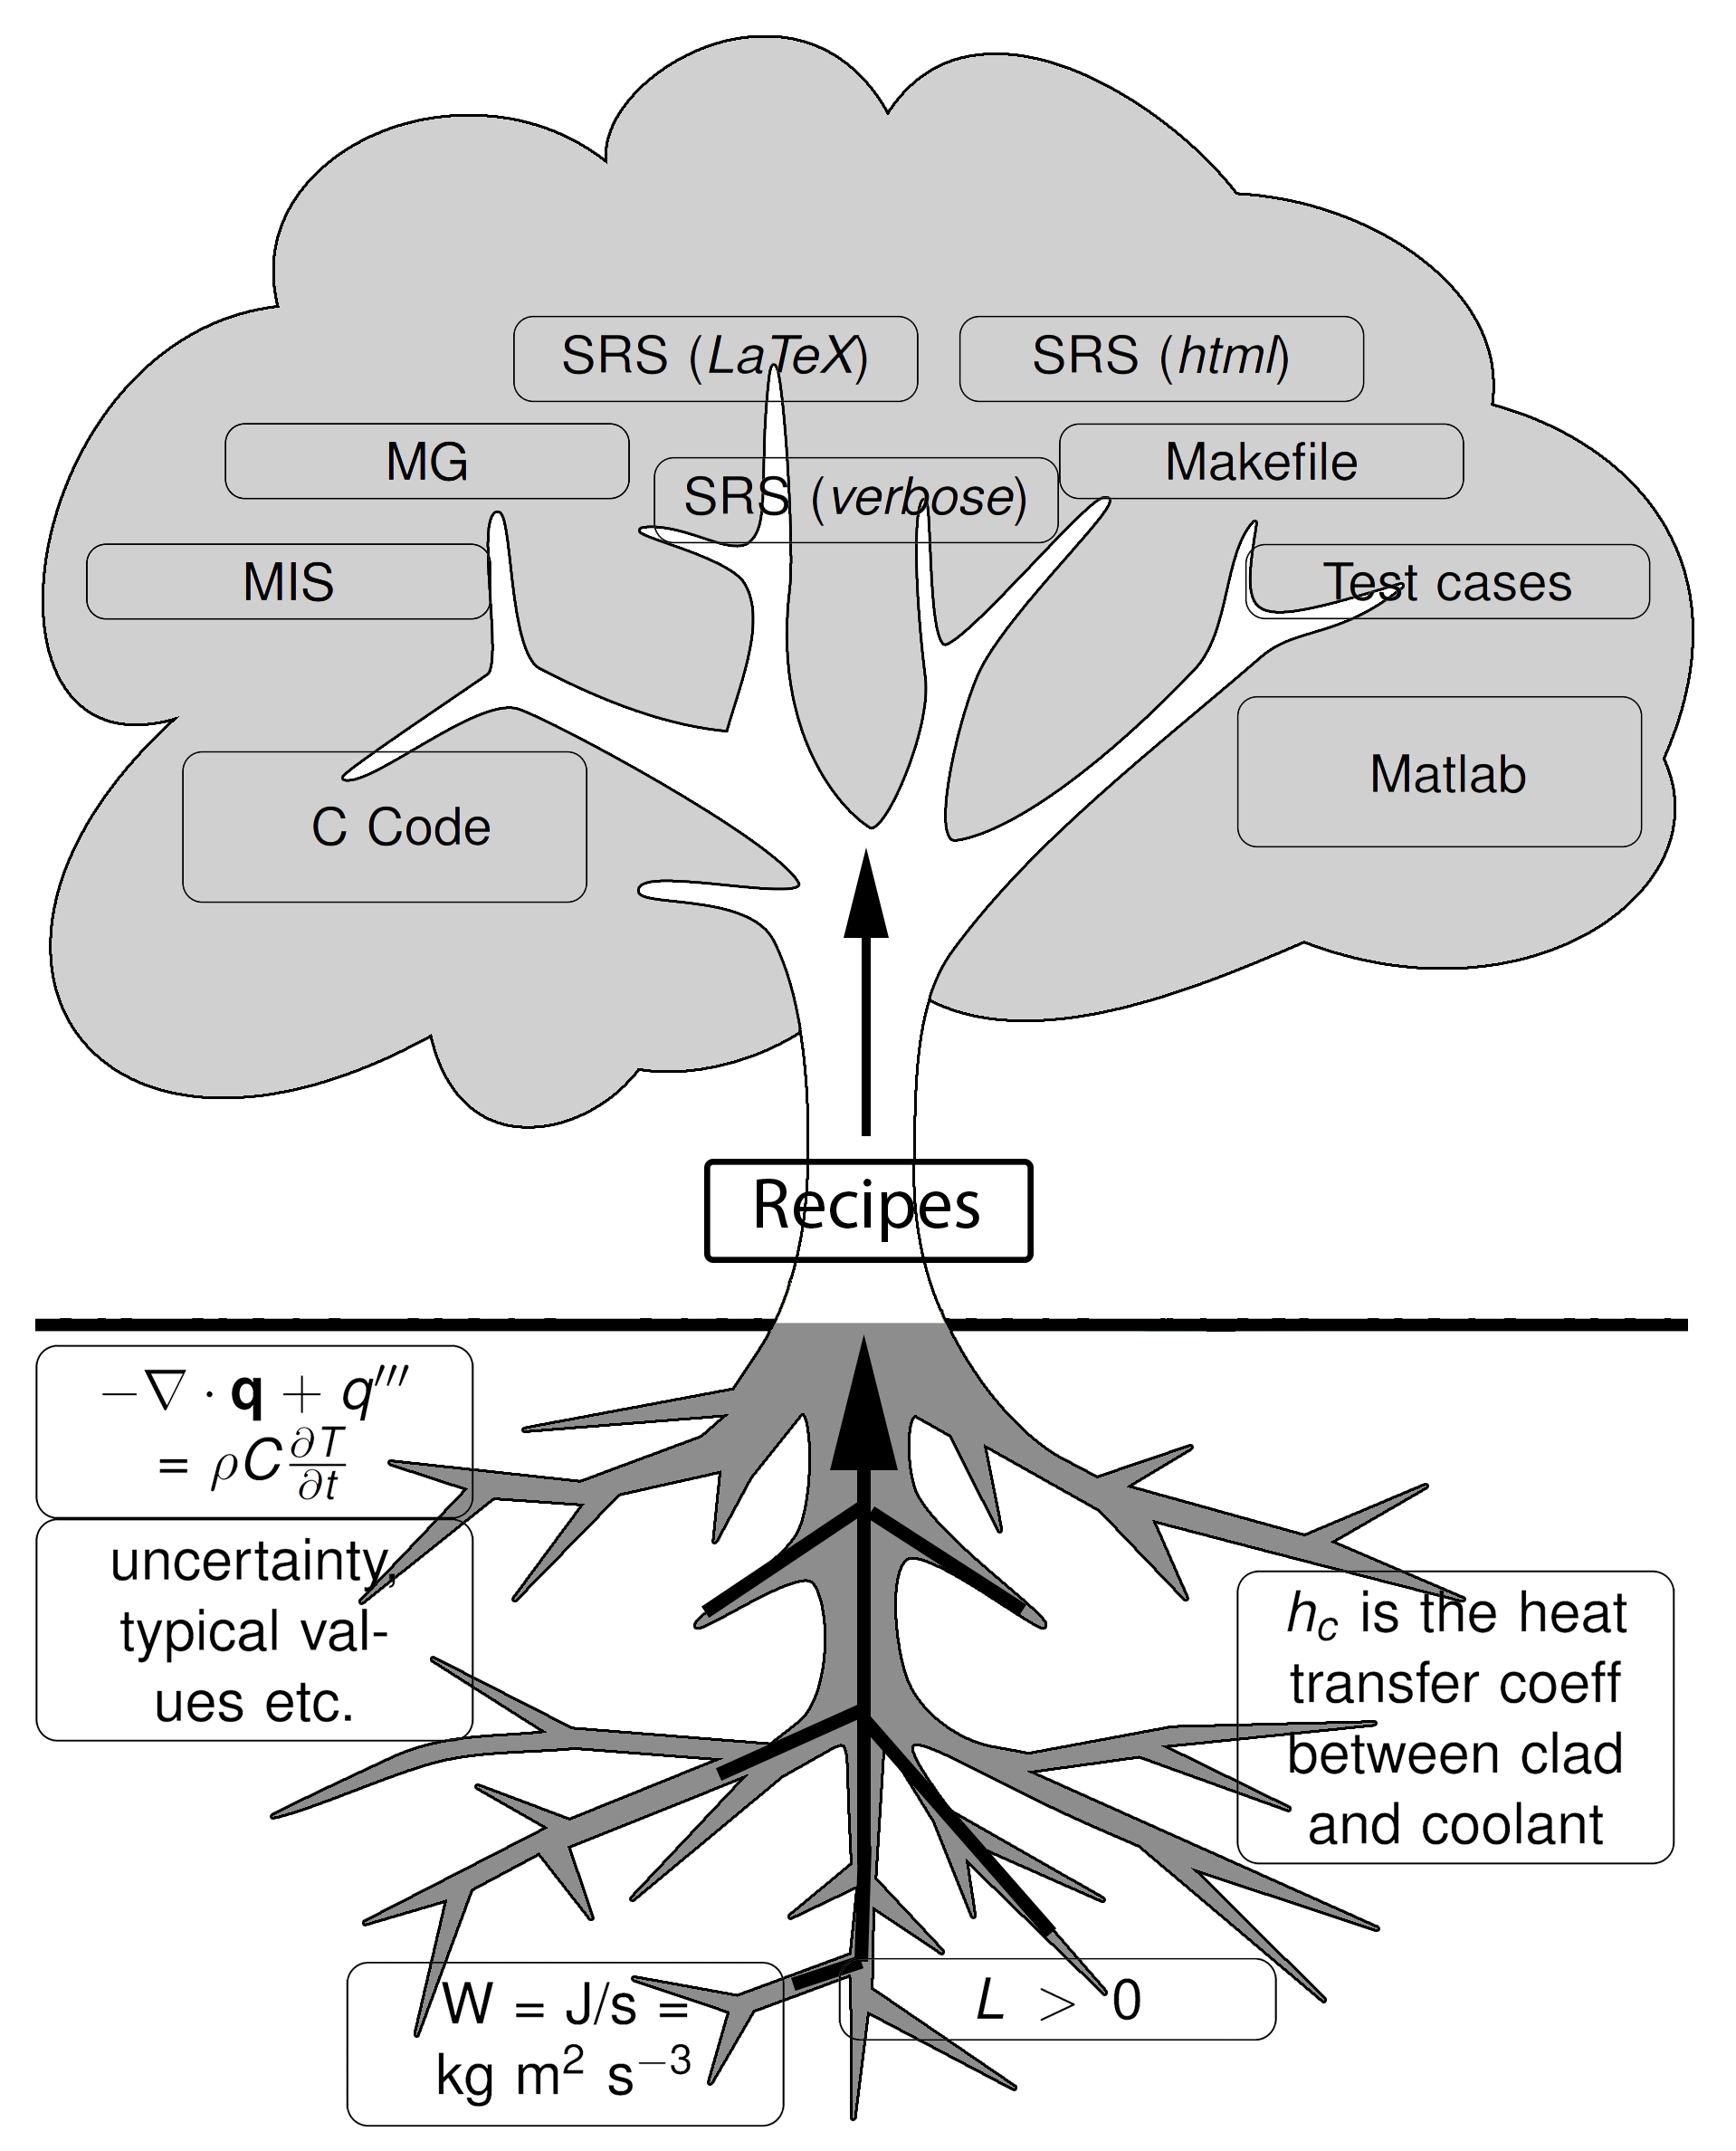
\includegraphics[width=0.8\textwidth]{tree.png}
\caption{Drasil concept}
\label{Fig:KnowTree}
\end{figure}

To clarify, Drasil is a framework for capturing knowledge and generating 
software from that knowledge. Our aim with Drasil is to generate \emph{all the 
things} -- i.e. all software artifacts including, but not limited to, the SRS, 
MG, MIS, test cases, build instructions, and source code -- from a single 
knowledge-base. To that end we have leveraged our experience with generative 
programming to create a number of Domain-Specific Languages (DSLs) to help 
achieve our goals. In the simplest terms, we use a DSL for knowledge-capture, 
document layout, printing, code-generation, and more. These will be discussed 
in more depth in Section~\ref{S:DrasilKC}.

Drasil's development has followed a cyclic approach of analysis and abstraction 
to reach its current state. We use our case studies as a guide, treating them 
like data, to search for commonalities. Once a commonality is found, we 
abstract it out and repeat the process. This approach allows for rapid progress 
due to constant iteration, while also helping us to determine what is 
``meaningful'' knowledge in the case studies as opposed to boilerplate 
information. This process of analysis and abstraction is what led us to our 
first real recipe for generating documents using the SmithEtAl template: 
\texttt{Drasil.DocumentLanguage}. Again, we will discuss that in more detail in 
the coming sections.

One last thing to note regarding Drasil is our liberal use of Haddock. The vast 
majority of Drasil is documented within the comments of the source code and 
this documentation can be extracted by running \texttt{make docs} on the Drasil 
repository at \url{https://github.com/JacquesCarette/Drasil}.

\wss{I like the above description of Drasil.  It felt more focused than some of
  the other sections.}

\subsection{Knowledge Capture \& Transformations in Drasil}
\label{S:DrasilKC}

  - How is Knowledge Capture handled in Drasil? - chunks!
 - Refer to chunk hierarchy Figure~\ref{Fig:ChunkHierarchy}
 - Talk about some of the implementation details -- lenses!

We have already started to capture knowledge in several areas ... 
  \fgr{} Knowledge areas we have started to capture (See: SE-CSE paper)

What about transformations? In high-level terms, they are our recipes.
More specifically, recipes combine atomic knowledge 
transformations to describe software artifacts to our generator. Atomic 
transformations come in two flavours, projections or translations. A projection 
typically involves using a lens to extract the relevant portion of knowledge, 
while a translation can take knowledge in one form and convert it to another. 
For example, we can translate an equation into an English description by 
projecting out each of its symbols' definitions and combining them into a 
sentence or description block. An example can be seen 
Figure~\ref{Fig:GlassBRDDSRS}.

\subsection{The Generator}

  - Key components of the generator / renderer
- The generator
  - HTML and TeX rendering
  - GOOL for code
- Sentence and Document

\subsection{The Recipe Language}

- Recipe Language(s) -- Example in action Refer to:
  \fgr{} Drasil.DocumentLanguage
- System Information -> Get into it


\subsection{Packaging Drasil}

The current version (0.1.23 as of this writing) of Drasil is built as a group 
of Haskell packages (see Figure~\ref{Fig:Packages}). The core components, 
including those for document concepts, are stored in a package named \edl{} and 
code-related components are in \edc{}. The main generator code is in \edg{}, 
with the HTML and LaTeX printers in \edp{}. We maintain our current 
knowledge-base in \edd{} and our case study examples in \ede{}. Finally, we 
have our document recipes in \eddl{}.

\begin{figure}
\begin{tikzpicture}

%TODO: Fix this

\node (drasil-lang) [class] {\dl};
\node (drasil-code) [class, below left=1 and 0.2cm of drasil-lang] {\dc};
\node (drasil-data) [class, below right=1 and 4cm of drasil-code] {\dd};
\node (drasil-example) [class, below left=1 and 0.54cm of drasil-data] {\de};
\node (drasil-printers) [class, below right=1 and 1cm of drasil-lang] {\drp};
\node (drasil-gen) [class, below left=of drasil-printers] {\dg};

%lang coords
\coordinate [above=2.785cm of drasil-data] (rightl);
\coordinate [above=1.28cm of drasil-code] (leftl);
%code coords
\coordinate [below=1.25 of drasil-code] (underc);
\coordinate [below left=1.53 and 0.5 of underc] (underleftc);
\coordinate [left=0.5 of drasil-code.south] (leftc);
%data coords
\coordinate [below=1.285 of drasil-data] (underd);

%code
\draw [myarrow] (drasil-code.north) -- (leftl) -- (drasil-lang.west);

%data
\draw [myarrow] (drasil-data.north) -- (rightl) -- (drasil-lang.east);
\draw [myarrow] (drasil-data.west)  -- (underc) -- (drasil-code.south);

%example
\draw [myarrow] (drasil-example.north) -- (drasil-lang);
\draw [myarrow] (drasil-example.west) -- (underleftc) -- (leftc) node[midway, 
left]{depends};
\draw [myarrow] (drasil-example.east) -- (underd) -- (drasil-data.south);

\end{tikzpicture}
\caption{Drasil package dependencies}
\label{Fig:Packages}
\end{figure}

\subsubsection{\dl}

The core language used within the Drasil framework, including all of the 
building blocks for our knowledge-base are stored within \edl{} under the 
exported module \texttt{Language.Drasil}. This package also exports a second 
module with functionality targeted to developers of Drasil known as 
\texttt{Language.Drasil.Development}.

\texttt{Language.Drasil} presently contains the expression DSL, document layout 
DSL, and knowledge capture classes \& data types. Every other \emph{drasil-*} 
package relies on, and builds off, this core.

With \texttt{Language.Drasil} alone we can capture knowledge for generating
artifacts nearly identical to those shown in Section~\ref{S:IntroCases}. 
However this is a much lower-level approach than we would like to use and could 
be seen as being akin to programming in a lower-level language like C, or 
perhaps even assembly. 

\subsubsection{\drp}

The printing DSL for HTML and LaTeX are stored here under the namespace 
\texttt{Language.Drasil.Printers}. These are the DSLs which translate Drasil 
specifications to the target language(s). Please note that the 
printers for source-code are kept in a separate location.

\subsubsection{\dc}

The code generation DSL used within the Drasil framework is stored here under 
the namespace \texttt{Language.Drasil.Code}. The code generation framework 
incorporates \emph{GOOL}, a Generic Object-Oriented 
Language~\cite{Costabile2012}, to give us the 
ability to target multiple languages -- C++, C\#, Objective C, Java, Lua, and 
Python.

\subsubsection{\dg}

The main generator functions used by Drasil are stored here under the 
\texttt{Language.Drasil.Generate} namespace. These functions are used to take a 
Drasil specification and transform them for use by the appropriate printers to 
generate the final output file(s). Both code and document generation are 
handled through function-calls found here.

The actual body of \edg{} is very small, consisting of only approximately 60 
lines of Haskell code, but generation would fail without it.

\subsubsection{\dd}

The knowledge-base common to all Drasil programs is curated and maintained 
within this package under the \texttt{Data.Drasil} name. Currently we have 
captured 
knowledge in a range of domains including, but not limited to, Computation, 
Education, Math, Physics, and Software. We have also captured meta-knowledge 
related to documentation, physical properties, and more.

A more detailed breakdown of \texttt{Data.Drasil} is given in 
Section~\ref{S:Data}.

\subsection{\ddl}

The \eddl{} package contains an example recipe, found in 
\texttt{Drasil.DocumentLanguage}, targeted at recreating the 
SmithEtAl SRS template\cite{SmithEtAl????}. %DS Gotta add the year.
This is currently our only recipe, however, \eddl{} will contain our future 
recipes as well (once they are created)

\subsubsection{\de}

All of the code required to generate artifacts for our case study examples is 
maintained in this one package. Each case study has a unique namespace 
containing everything, other than common knowledge from \edd{}, required to 
generate that particular case study's artifacts. These namespaces can be seen 
in Table~\ref{Tab:Namespaces}. 

\begin{table}
\caption{Case study namespaces in \ede{}}
\label{Tab:Namespaces}
\begin{tabular}[]{ l | l}
		Case Study 		& 				Namespace 						\\
\hline{}
		GlassBR 		& 	\texttt{	Drasil.GlassBR			} 		\\
\hline{}
		GamePhysics 	& 	\texttt{	Drasil.GamePhysics		}	 	\\
\hline{}
		SSP 			& 	\texttt{	Drasil.SSP				}		\\
\hline{}
		SWHS 			& 	\texttt{	Drasil.SWHS				}		\\
\hline{}
		NoPCM 			& 	\texttt{	Drasil.NoPCM			} 		\\
\hline{}
		Tiny 			& 	\texttt{	Drasil.HGHC				} 		\\
\end{tabular}
\end{table}

\wss{I like the explanation of the packages}

\section{Case studies - in more depth}

- Re-introduce case studies
  - Our methods for reimplementing
  - CI for testing
- Start showing off re-use and automated generation.
  - Start with common knowledge (generalized \fgr{}?)
  - Then onto GlassBR example to show off the doc lang recipe (\fgr{}?)
  - Then let's see SRS vs. NoPCM for reuse (particularly NoPCM) (\fgr{}?)

\wss{I like how specific this section is.  You are highlighting specific
  lessons/findings from actual examples.  When you get stuck with writing other
  sections, this would be a good place to focus your energy.  You should be able
  to write this material almost independently of the other sections, at least to
  get started.}

\subsection{Data.Drasil}
\label{S:Data}

- Common knowledge
  \fgr{} SI\_Units
  \fgr{} Thermodynamics (ConsThermE?)

Important to not we have not captured even a minute fraction of all the domain 
knowledge, yet the results with out limited knowledge-capture already speak for 
themselves.

\subsection{GlassBR}

- Brief intro to problem GlassBR is solving - how it works
- Show off the doc language here
  \fgr{} GlassBR SRS in (truncated) DocLang format 
  - "Reads like a table of contents, with a few quirks"
- Show off some code generation
  \fgr{} Side-by-side of Chunk Eqn vs. Doc Eqn vs. Code 
  - "Easy to see that the code matches the equations"
- Talk about potential variabilities and how to make this a family
- Why is this interesting?
	- Fairly straightforward example of something a scientist would create/use 
	in their research

\subsection{NoPCM \& SWHS}

- Re-introduce the problems
- See how they're a family?
- Really drill in the similarities
  \fgr{} Figure showing NoPCM import(s)
- Lots of knowledge-reuse
- Very few 'new' chunks (count them?)
- Show example of variability in action
  \fgr{} Equation with/without PCM (rendered?)
- Why this example is interesting:
  - ODE solver -> We don't gen, just link to existing good one(s)

\subsection{Others}

- Mention SSP, Tiny, GamePhysics, but don't go too in-depth.
  - Useful examples as they give us a wider range of problems for analysis
- Testing
  - Physics is physics -> when we make updates, the underlying knowledge isn't
    changing, so neither should our output
  - Refer to CI

\section{Results}

- Here we discuss the results we've seen so far.
- Had some of these case studies attempted to be certified, they would (should) 
have failed.
	- A number of common problems.

\wss{I like this Results section - examples like these are something people can
  understand and hopefully be convinced by.}

\subsection{Common issues across case studies}

Across all of our case studies we were able to find a number of undefined 
symbols using Drasil. This was after multiple passes by humans attempting to 
ensure the documents were consistent and up-to-date had failed to catch these 
small, but important, missing pieces of knowledge. 

Drasil was able to detect and correct the issues through its automated 
generation of the symbol table and use of sanity-checking to ensure that any 
symbol used had to have been defined within the table of symbols to be used 
elsewhere in the artifacts.

The symbols that lacked definitions were typically those with an ``understood" 
meaning in the context of their domain, but not once did that definition appear 
concretely in any of the software artifacts.

\wss{You are giving specific examples below, right?}

\ds{Yes.}

\subsection{NoPCM and SWHS}

- Along with the common errors, there was some sharing of PCM-related knowledge
  - Found because PCM symbols were not in the ToS and the sanity-check caught 
  it.
  - No way to specifically exclude knowledge that shouldn't 'exist' in a project
- Work in Kolmogorov complexity / MDL for NoPCM + SWHS?
- Kolmogorov/MDL implies less writing for the same artifacts -> less to sift 
through = maybe better? Need to run experiments to know for sure.

\subsection{SSP}

- Symbols for given quantities changed throughout the documentation
  - Went unnoticed by a human for years! Found almost instantly by Drasil
    - the new symbols were undefined.

Immediately improved the quality of the documentation, particularly in terms of 
consistency!

\subsection{Pervasive Bugs}

One of the utmost benefits of the knowledge-based approach using Drasil is the 
introduction of ``pervasive bugs". These are typically mistakes made in the 
captured knowledge which propagate across all generated artifacts wherein that 
knowledge is used. Calling this a benefit may seem counter-intuitive, but when 
an error appears in a multitude of locations it is far more likely to be caught 
then if it were hiding in the corner of one artifact.

Not only is it more likely that we will find an error, it is also far easier to 
track down the source of said error -- we need only go to the knowledge base 
and find the requisite chunk. We can also tune error messages to point us at 
the offending chunk if we so desire.

Correcting an error in a chunk of knowledge is also trivial. It only needs to 
be fixed once to be fixed across all of our software artifacts. No need to 
\texttt{grep}, find-and-replace, or the like.

\subsection{Freebies - Compliments of System Information}

- Thanks to the recipe language and the way we structure out system information
  we can get
- Table of Symbols
- Table of Units
- Table of Abbreviations and Acronyms
- Bibliography

\begin{figure}
\caption{Tiny before (left) and after (right) use of Document Language and 
System Information}
\end{figure}

- All tedious to do by hand, but are free to automatically generate
- Generator includes sanity-checking -> Can't use something that isn't defined!
- Sanity-checks are 'free' -> we can check for errors with our symbols,
  ensure units are consistent, guard against constraints, and ensure we only
  reference those things which are defined in our system. 
- Sanity-checks are run every time artifacts are generated.

\subsection{Improved Understanding of Software Artifacts}

%TODO: Fill in
- Another benefit to using Drasil for writing recipes and performing 
knowledge-capture is the increased 
understanding of software artifacts that follows. To write a recipe, one needs 
to truly understand what is being said and how each piece of knowledge relates 
to each other. 

[*SS* - Related to the previous \ds{now next} point, the act of formalizing the 
knowledge that
goes into the requirements documentation forces us to deeply understand the
distinctions between difference concepts, like scope, goal, theory, assumption,
simplification, etc.  With this knowledge we can improve the focus and
effectiveness of existing templates, and existing requirements solicitation and
analysis efforts.  Teaching it to a computer.]

\section{Future Work}

[*SS* - Once we are capable of true variability in the documentation, we can
really start asking the question about what is the "best" documentation for a
given context.  In the future experiments could be done with presenting the same
information in different ways to find which approach is the most effective.]

- Run an experiment to determine how easy it is to create new software with 
Drasil.

- Run an experiment to see how easy it is to find and remove errors with Drasil

- Experiment to see time saved in maintenance while using Drasil vs. not

- Design language

- Open issues (as of writing there are \#\#\# %DS 147
issues currently open on the Drasil repository).

- User friendliness

\section{Conclusion}

- Easier to find errors (anecdotally) - future work will tell us if this holds.

It is not (yet) faster or easier to create software using Drasil, however, we 
front-load the investment of effort and receive a number of benefits. 
Consistency by construction is paramount! 

The next step, experimentation, is pivotal to confirm our intuition holds and 
hopefully show a knowledge-based approach with strong tool-support is feasible 
for software family generation.

\bibliography{drasil}
\bibliographystyle{acm}
\end{document}
